\PassOptionsToPackage{uline}{hhtensor}
\PassOptionsToPackage{table}{xcolor}

\documentclass[a4paper,oneside,reqno,onecolumn]{amsart}

\input{../cambridge-macros.tex}

\newcommand{\U}{\matr{U}}
\newcommand{\V}{\matr{V}}
\newcommand{\W}{\matr{W}}
%\newcommand{\x}{\vec{x}}
\newcommand{\m}{\vec{m}}
\newcommand{\s}{\vec{s}}
\renewcommand{\o}{\vec{o}}
\DeclareMathOperator*{\softmax}{softmax}


%    Set assignment information here
\newcommand{\authorname}{Feynman Liang}
\newcommand{\coursename}{MLSALT: MPhil Thesis}
\newcommand{\assignmentname}{BachBot: Generative music modelling using LSTMs}

\begin{document}

\title{\coursename\\\assignmentname}
\author{\authorname}
\email[A1]{fl350@cam.ac.uk}
\address[A1]{Churchill College}
\date{\today}

\begin{abstract}
Lorem ipsum
\end{abstract}

\maketitle

\tableofcontents

\section{Introduction}

Algorithmic composition is the application of a well-defined algorithmic
procedure to compose music.

An interesting question regarding creativity: if an algorithm faithfully reproduces
an artist's creative process, what is the difference between music produced by the artist
and music produced by the algorithm?

\section{Background}

\begin{quote}
    The overwhelming majority of these state-of-the-art systems address a benchmark
task by applying linear statistical models to ad-hoc features. In other words, the
researchers themselves discover intermediate representations by engineering task-specific
features. These features are often derived from the output of preexisting systems, leading
to complex runtime dependencies. This approach is effective because researchers leverage
a large body of linguistic knowledge. On the other hand, there is a great temptation to
optimize the performance of a system for a specific benchmark. Although such performance
improvements can be very useful in practice, they teach us little about the means to progress
toward the broader goals of natural language understanding and the elusive goals of Artificial
Intelligence.
\end{quote}\cite{Collobert2011}

\subsection{Data Representation}

We are interested in modelling the transcription of a musical composition.

We consider note duration, time, and velocity. We neglect changes in timing
(e.g. ritardandos), dynamics (e.g. crescendos), and stylistic notations (e.g.
accents, staccatos, legatos).

\todo{Do we consider note velocities? key/time signature metadata?}

\emph{Piano roll} music transcriptions are quantized both in time ($t \in T$)
and note frequencies ($n \in N$). frequencies quantized to a piano roll.
\todo{Motivate quantization with Western music}.

We can represent a piano roll transcription as a high-dimensional vecctor
$X_{t,n} \in \RR^{|T| \times |N|}$ where $X_{t,n}$ denotes the note velocities
for note $n$ at time $t$.

\subsubsection{Psychoacoustic Features and Gray Codes}

Aware, unused.

\subsubsection{Input preprocessing}

\begin{enumerate}
    \item Transpose to Cmaj/Amin
    \item Strip all dynamics info
    \item Restrict to 4/4
\end{enumerate}

\subsection{Neural Network Sequence Modeling}

\subsubsection{Feedforward Neural Network}

Increasing context window size is not always a good solution:
\begin{itemize}
    \item Too small $\implies$ no long-term dependencies captured
    \item Not all $N$-grams observed $\implies$ need back-off and discounting
\end{itemize}

How do we handle variable length inputs?

\subsubsection{Recurrent Neural Networks}

Carry memory $s_t$ through time $t$, ``summary of infinite context duration
i.e.\ all previously processed data''

Share weights $\matr{U}, \matr{V}, \matr{W}$ over $t$ since performing same
task at each time i.e.\ modeling $P(o_t | s_t, x_t) = \softmax(V s_t)$.

\begin{figure}[htpb]
    \centering
    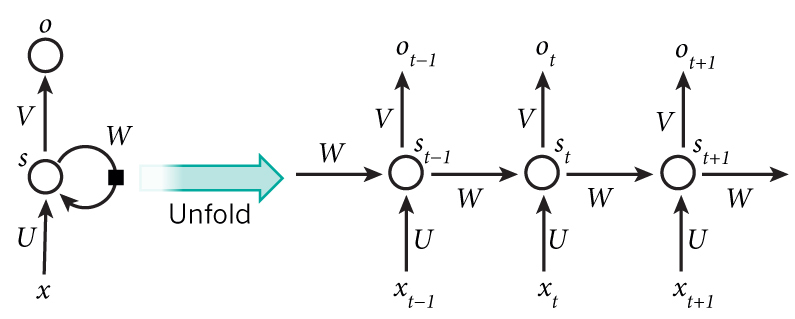
\includegraphics[width=0.8\linewidth]{Figures/rnn.jpg}
    \caption{\todo{Redraw in xy}}
\end{figure}

\begin{align}
    \s_t &= f(\U \x_t + \W \s_{t-1}) \\
    \o_t &= \softmax( \V \s_t)
\end{align}

$f$ is usually $\tanh$ or ReLU.

\begin{enumerate}
    \item Memory/state $\s_t$ summarizes ALL previous information
    \item $\U, \V, \W$ parameters are shared across all $t$. Reflects
        that the same task is being performed at each input i.e.\
        invariance over time. Reduces number of parameters.
\end{enumerate}

\subsubsection{Applications of RNNs}

\begin{enumerate}
    \item Language modeling
        \begin{enumerate}
            \item Model $P(\m), \m \in V^T, T \in \NN$
            \item Train to predict the distribution of the next note in the
                melody i.e.\ $\o_t = P(\m_t | \m_{1:t-1})$
            \item $\m_{t-N:t-1}$ is given explicitly as input $\x_t$ and
                $\s_{t}$ captures information from before $t-N$
            \item See \cite{Martens2011}, \cite{Mikolov2011}, \cite{Mikolov2010}
        \end{enumerate}
    \item Machine translation
        \begin{enumerate}
            \item~\\
                \begin{figure}[htpb]
                    \centering
                    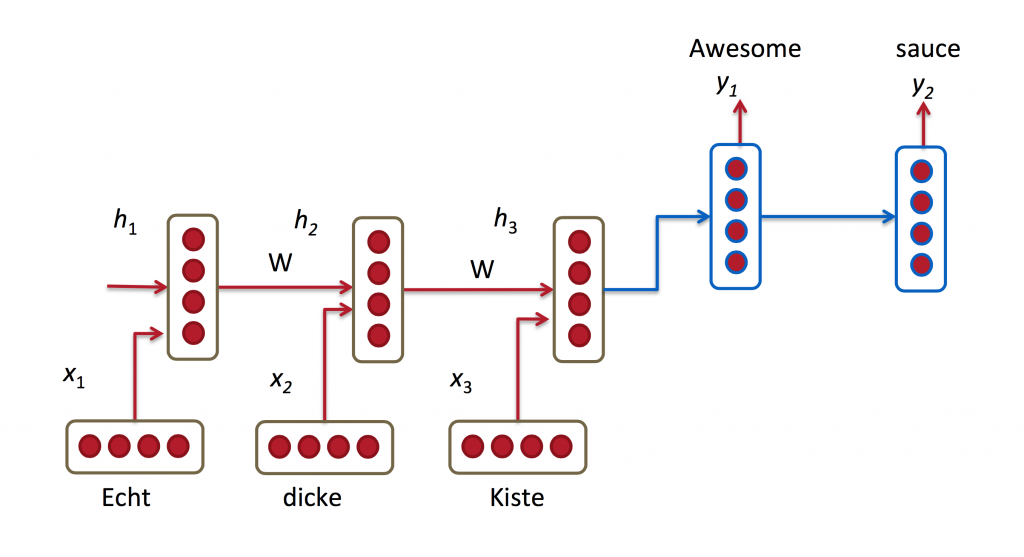
\includegraphics[width=0.8\linewidth]{Figures/rnn-mt.png}
                    \caption{\todo{Redraw in xy}}
                \end{figure}
            \item Input is a sequence of words in source language $\leftrightarrow$
                sequence of notes in $V$
            \item Output is four sequences of notes, one for each of the 4 chorale parts.
            \item Architecture difference: output only starts after input is completely
                consumed because first word of translated sentence may require information
                from complete sentence input
                \begin{enumerate}
                    \item This could be mitigated with bidirectional LSTMs \cite{Graves2005}
                    \item Could also try Neural MT \cite{Bahdanau2015}, whose attention
                        neural network could be used to extract insights about which parts
                        of the overall melody influences decision making within local regions
                        of music
                \end{enumerate}
            \item See \cite{Liu2014}, \cite{Auli2013}, \cite{Sutskever2014}.
        \end{enumerate}
\end{enumerate}

\subsubsection{RNN Extensions}

\begin{enumerate}
    \item Bidirectional RNNs
        \begin{figure}[htpb]
            \centering
            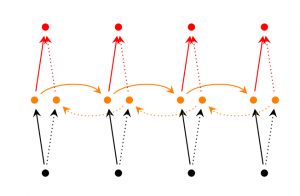
\includegraphics[width=0.8\linewidth]{Figures/bi-rnn.png}
            \caption{\todo{Redraw}}
        \end{figure}
        Cannot be sampled, but if the source sequence is given can run FW and BW LSTMs
        to obtain $\s^{FW}$ and $\s^{BW}$ then $\o_t = \softmax(V [\s^{FW}_; \s^{BW}_t])$
    \item Deep RNNs
        \begin{figure}[htpb]
            \centering
            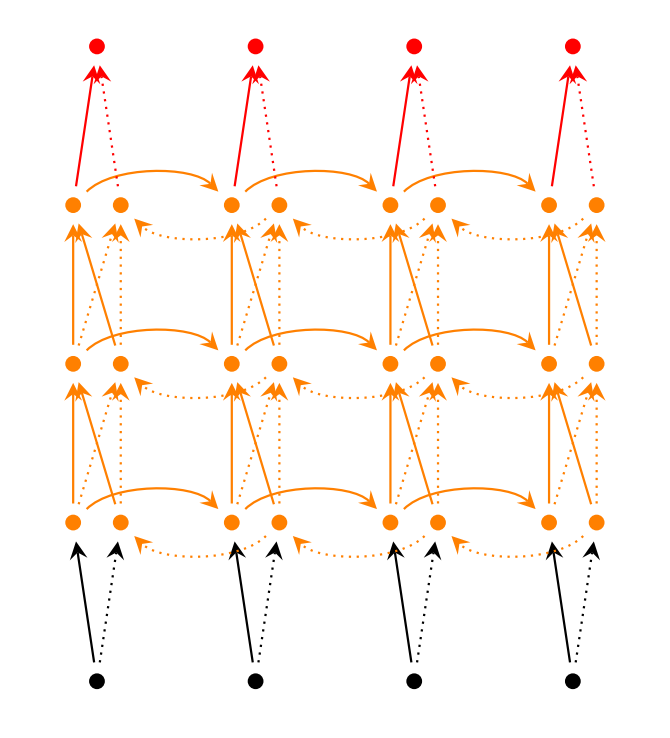
\includegraphics[width=0.8\linewidth]{Figures/deep-rnn.png}
            \caption{\todo{Redraw}}
        \end{figure}
        Outputs of one LSTM are used as inputs to the next; more layers $\implies$
        greater representational power, hierarchical representation learning?
    \item LSTMs
        \begin{enumerate}
            \item Memory is called \emph{cells}
            \item 
        \end{enumerate}

    \item LSTM Variants: GRUs have fewer parameters (U and W are smaller) and
        thus may train a bit faster or need less data to generalize
\end{enumerate}

\subsection{Invariances}

Music should be relatively invariant to transpositions in frequency.

\subsection{Music Theory}

\subsubsection{Composition Types}

\begin{itemize}
    \item Chorale
    \item Fugure
    \item \todo{FILL IN}
\end{itemize}

\subsubsection{Network connectivity}

\section{Research Goals}

Following the natural process undertaken by many human composers, we divided
the music generation task into two subproblems:
\begin{enumerate}
    \item Generating a melody line $\vec{m}$
    \item Given a fixed melody line, generate the four voices $\{\vec{v}_i\}_{i=1}^4$
\end{enumerate}

Sample a melody m $\sim$ P(m) where P(m) is given by a LSTM, then load up 4
encoder/decoder biLSTMs (one for each voice) with m and get their MAP outputs

\subsection{Monophonic Modeling}

Equivalent to language modeling problem. Goal is to model $P(\vec{m})$ for $\vec{m}
\in V^T$, $T \in \NN$. LSTM architecture can capture longer range dependencies.

\subsection{Polyphonic Modeling}

Can be interpreted in machine translation as translation from source language $\vec{m}$
to multiple target languages $\vec{v}_i$.

\section{Experiments}

\subsection{Data formant and preprocessing}

We use the kern file format, strip header information, replace measure counts
with a \texttt{@} symbol for measure delimiters.

\subsection{Monophonic generation}

We first attempt to model the single melody line of a chorale.

\subsubsection{Melody extraction}

One method is to use the soprano line as the melody.

\todo{Annotations?}

\subsubsection{Single voice LSTM training}

\subsection{Polyphonic generation}

\subsubsection{Generating harmony for single voice}

\subsubsection{Bidirectional LSTM}

\bibliographystyle{alpha}
\nocite{*}
\bibliography{refs.bib}

\onecolumn

\appendix

\section{Code listings}

\end{document}

